%--- 1 ----------------------------------------------------------
\item\qouv{Définissez ce qu’est un design pattern, comment le caractériser et à quoi il sert.}
{Un design pattern est un \textbf{modèle de conception} général qui répond à une problématique récurrente en développement. Il s'agit d'une desciption de solution dont l'implémentation doit être adpatée aux cas particulier.
\paragraph{}
Les patterns sont donc utilisés pour simplifier la vie des programmeurs, ils représentent un gain de temps (ne pas réinventer la roue) et une fiabilité puisqu'ils s'agit de modèles testés et approuvés avec le temps.

\paragraph{}
Un pattern est définit par:
\begin{itemize}
\item[$\cdot$]un \textbf{nom}
\item[$\cdot$]une \textbf{description du problème} auquel il s'applique
\item[$\cdot$]la \textbf{solution}: générique!! Son implémentation est à adapter au cas par cas
\item[$\cdot$]les \textbf{conséquences} de son utilisation: peut avoir des répercutions sur le reste du code, forcer des choix d'implémentation allieurs,...
\end{itemize}

\paragraph{}
Il existe 23 patterns \textit{classiques}, définis par le GoF, regroupés selon trois catégories:
\begin{enumerate}
\item \textbf{construction}: concerne l'instanciation des classes
\item \textbf{structuraux}: concerne l'organisation des classes entre elles
\item \textbf{comportementaux}: concerne la communication entre les objets
\end{enumerate}
}

%--- 2 ----------------------------------------------------------
\item\qouv{Que sont les concurrency patterns ? Donnez quelques exemples.}
{Ce sont des patterns utilisés pour de la \textbf{programmation concurrente}.
Ils apportent entre autre des modèles pour: la synchronisation, la communication, le stockage de données, les caches,...\paragraph{EXEMPLES [...]}
}

%--- 3 ----------------------------------------------------------
\item\qouv{Décrire ce qu’est le test driven development (TDD).}
{Le cycle TDD définit une méthode de développement qui consiste à être \textbf{guidé par l'écriture de tests} et intégrer des phases de refactoring.
\paragraph{}
La figure ci-dessous définit les trois grandes étapes de chaque tour de cycle. La deuxième étape consiste à écrire un code permettant de passer le(s) test(s) -> on ne parle encore d'optimisation. C'est seulement à l'étape 3, lorsque le code est fonctionnel, que l'on peut penser à des améliorations pour éliminer les \textit{bad smells}.
\begin{figure}[h!]
\center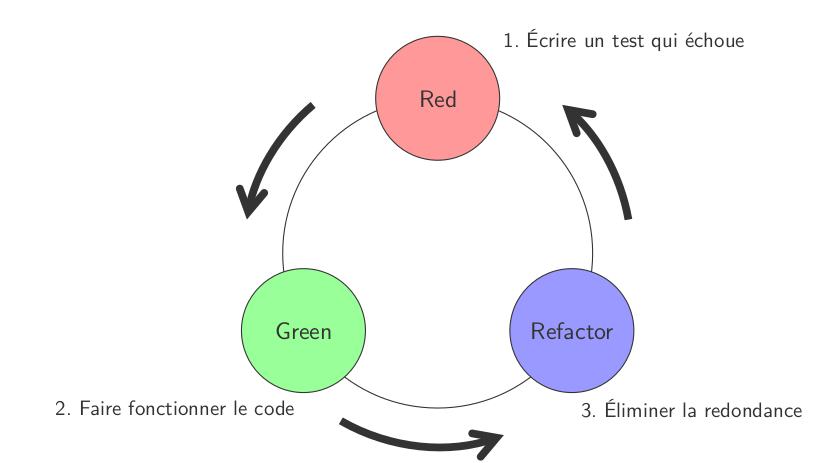
\includegraphics[scale=.4]{images/cycle-tdd}
\caption{Le cycle TDD selon Kent Beck}
\end{figure}

}

%--- 4 ----------------------------------------------------------
\item\qouv{Définissez ce qu’est un bad smell et donnez un exemple.}
{Un \textit{bad smell} est une \textbf{faiblesse de codage} dans un programme, il ne s'agit pas d'un bug!!!
\paragraph{}Exemples de bad smells:
\begin{itemize}\setlength{\itemsep}{.3em}
\item[$\cdot$] \textbf{Large class (the blob)}: une classe (God class) monopolise tout le traitement et les autres stockent uniquement des données -> va à l'encontre du principe de POO "une classe = une responsabilité". La \textit{God Class} utilise des détails d'implémentation des autres classes -> va à l'encontre de l'encapsulation.
\item[$\cdot$]\textbf{code dupliqué}: du code identique ou très similaire à différents endroits dans le programme -> difficile à maintenir. Il faut isoler les parties communes dans des métodes.
\item[$\cdot$]\textbf{Long method}: méthode dont le coprs possède beaucoup d'instructions -> limite la réutilisabilité et difficile à comprendre. Une méthode ne devrait avoir qu'une seule fonctionnalité.
\item[$\cdot$]...
\end{itemize}
}

%--- 5 ----------------------------------------------------------
\item\qouv{Définissez ce qu’est le refactoring et à quel moment il peut être utilisé dans le processus de
développement.}
{Le refactoring consiste à transformer du code tout en \textbf{préservant son comportement}, il s'agit donc d'\textbf{améliorer la qualité} d'un code déjà fonctionnel.
\paragraph{}
Cette technique s'inscrit dans la logique d'\textit{optimisation du code}, dont un principe fondamental est le suivant: \textit{"l'optimisation ne doit intervenir qu'une fois que le programme fonctionne et répond aux spécifications fonctionnelles."}
\paragraph{}
Dans le cas d'un cycle TDD (Test-Driven Development, voir Q3), le réfactoring du code a donc lieu après que celui-ci ait passé une batterie de tests. L'idée est de se servir de ces mêmes tests pour s'assurer que les modifications n'aient pas altéré le bon fonctionnement du code.

\paragraph{EXEMPLES [...]}

\paragraph{Remarque: }
l'étape de refactoring n'ajoute pas de fonctionnalité et ne corrige pas de bug !! On re-travaille un code dans le but d'améliorer sa lisibilité et sa maintenance mais son comportement externe reste identique.

}

%--- 6 ----------------------------------------------------------
\item\qouv{Définissez la notion de paradigme de programmation, ainsi que la programmation impérative et
déclarative.}
{Un paradigme est une représentation du monde, une manière de voir les choses, un modèle cohérent qui repose sur une base définie.
\paragraph{} \setlength{\itemsep}{.3em}
Dans le domaine de l'informatique, un paradigme de programmation est:
\begin{itemize}
\item[$\cdot$]un \textbf{style fondamental} qui traîte de la manière dont les solutions aux problèmes doivent être formulées dans un langage de prog.
\item[$\cdot$]une \textbf{manière de programmer} un ordinateur, basée sur un ensemble de principes ou une théorie
\item[$\cdot$]un \textbf{ensemble de concepts} particulier
\end{itemize}

\paragraph{}
Définitions des paradigmes \textit{impératif} et \textit{déclaratif} aux questions V/F 17 et 18.


\paragraph{Exemples...} une façon de voir les choses du monde réel est de les modéliser au moyen d'objets/patrons avec des caractéristiques et la possibilité de les traîter, ce qui a amené au paradigme de la POO. \paragraph{}Dans d'autres cas, on préférera l'utilisation de fonctions mathématiqes établies auxquelles ont fournit des paramètres, d'où le paradigme de prog. fonctionnelle.\paragraph{}Ou encore, on peut utiliser un programme pour établir une séquence d'instructions qui changent l'état de ses variables, ce qui correspond à un modèle impératif.
}


%--- 7 ----------------------------------------------------------
\item\qouv{Définissez la notion de système distribué en reprenant rapidement les cinq buts.}
{"L’architecture d'un environnement informatique ou d'un réseau est dite distribuée quand toutes les ressources ne se trouvent pas au même endroit ou sur la même machine." - \textit{Wikipédia}
\paragraph{}
Dans une telle architecture, les composants sont répartis sur plusieurs plateformes, matérielles (machine, serverus,...) ou logicielles (machine virtuelle,...), et coopèrent via un \textbf{réseau de communication} (ethernet, wifi, mémoire partagée,...).
\paragraph{}
Les buts principaux de l'architecture distribuée sont les suivants:
\begin{enumerate}\setlength{\itemsep}{.3em}
\item la TRANSPARENCE: pour l'utilisateur, le système doit apparaître comme un \textbf{unique système cohérent}, il faut que l'ensemble des machines engagées apparaissent comme une seule. \paragraph{}Cet aspect de "transparence" peut être considéré à différents niveaux:
	\begin{itemize}\setlength{\itemsep}{.2em}
	\item[$\cdot$] \textcolor{ltred}{\textsc{accès aux ressources}}: la façon dont les ressources sont accédées doit être cachée
	\item[$\cdot$] \textcolor{ltred}{\textsc{localisation des ressources cachée}}: il ne faut pas dépendre du lieu ou sont les ressources
	\item[$\cdot$] \textcolor{ltred}{\textsc{présence de différentes technologies}}: différents OS, langages, frameworks,... doivent pouvoir "cohabités" dans le système sans l'impacter
	\item[$\cdot$] \textcolor{ltred}{\textsc{migration des ressources}}: une ressource doit pouvoir être changée d'emplacement
	\item[$\cdot$] \textcolor{ltred}{\textsc{réplication des ressources}}: une même ressource peut se trouver sur plusieurs composants en même temps
	\item[$\cdot$] \textcolor{ltred}{\textsc{concurrence entre plusieurs utilisateurs}}: un utilisateur utilise le système comme s'il était le seul, il n'a pas conscience de la présence des autres et les ressources doivent donc pouvoir être partagées entre eux
	\item[$\cdot$] \textcolor{ltred}{\textsc{panne et défaillance de ressources}}: un problème technique ne doit pas être ressenti par l'utilisateur
	\item[$\cdot$] \textcolor{ltred}{\textsc{persistence}}: cacher le fait qu'une ressource se trouve en mémoire ou sur le disque
	\end{itemize}
\item l'OUVERTURE: le système offre des services en suivant un \textbf{standard} afin de simplifier sa construction et les changements futurs. De cette façon, une machine pourra facilement être rajoutée au système, peut importe ses caractéristiques, tant qu'elle respecte le standard. On obtient ainsi un ensemble \textbf{hétérogène} de machines
\item la FIABILITE: un système distribué étant plus difficile à mettre en oeuvre, il doit être plus efficace/fiable que son équivalent en centralisé unique
\item la PERFORMANCE: l'architecture distribuée doit augmenter les performance du système. Grâce à l'hétérogénétié du système, il est possible de combiner des machines spécialisées dans le traîtement de certaines tâches
\item l'EVOLUTIVITE: le système doit pouvoir évoluer facilement, il faut pouvoir ajouter des ressources et ce de  façon dynamique, pendant l'exécution. Une machine ajoutée au système doit être reconnue directement par les autres et intégrée à l'ensemble des opérations. Pour cela, elle envoie au réseau ses propres caractéristiques, suite à quoi elle se voit attribuer les tâches en fonctions de ses "compétences".
\paragraph{}
L'évolutivité doit permettre de faire face à deux principaux problèmes: 
	\begin{itemize}
	\item[$\cdot$] \textcolor{ltred}{\textsc{size scalability}}: augmenter le nombre de ressources pour éviter que le système ne surcharge
	\item[$\cdot$] \textcolor{ltred}{\textsc{geographical scalability}}: augmenter le nombre de ressources pour diminuer les délais de communication
	\end{itemize}
\end{enumerate}

\paragraph{}
Finalement, les avantages et inconvénients d'une telle architecture sont les suivants:
\begin{itemize}\setlength{\itemsep}{.3em}
\item[\textcolor{dkgreen}{\ding{52}}] économie de ressources: possibilité d'acheter des machines supplémentaires moins chères pour augmenter les capacités du système
\item[\textcolor{dkgreen}{\ding{52}}] augmentation de la vitesse et de la fiabilité: si une machine tombe en panne, le reste du système est établit pour ne pas perdre de donnée et éventuellement prendre les relais et continuer de fonctionner normalement
\item[\textcolor{dkgreen}{\ding{52}}] croissance incrémentale: ajout simple de machine
\item[\textcolor{dkred}{\ding{56}}] complexité logicielle et interopérabilité (hardware ou software): si le système est mal conçu, il sera fermé à l'extension. Ex: si trop de dépendance avec le hardware -> problèmes de compatiblités pour ajouter des machines
\item[\textcolor{dkred}{\ding{56}}] nécessité d'avoir un réseau de communication
\item[\textcolor{dkred}{\ding{56}}] sécurité plus difficle à garantir sur l'ensemble du système
\end{itemize}


}

%--- 8 ----------------------------------------------------------
\item\qouv{Définissez la notion de middleware. Dans quel type d’architecture les retrouve-t-on ?}
{"Un middleware est un logiciel tiers qui crée un réseau d'échange d'informations entre des applications." - \textit{Wikipédia}
\paragraph{}
Il permet à des apps hétérogènes, qui ne sont pas prévues pour se "parler", de communiquer ensemble via une même technique d'échange d'informations.
\paragraph{}
Il supporte l'architecture distribuée: les applications peuvent donc se trouver sur des machines différentes et s'échanger des informations quels que soient les ordinateurs impliqués et les caractéristiques matérielles/logicielles. 
\paragraph{}
Le middleware agit donc comme un buffer entre les applications et le réseau. 

\begin{figure}[h!]
\center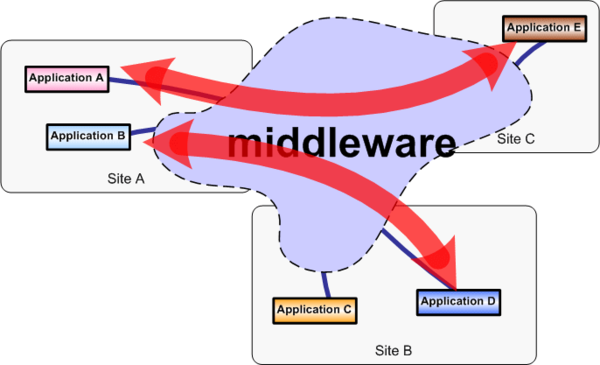
\includegraphics[scale=.4]{images/middleware}
\caption{Schématisation d'un middleware en réseau distribué \cite{ref8}}
\end{figure}

\paragraph{}
L'infrastructure middleware peut être décomposée en plusieurs couches:
\begin{enumerate}
\item couche de \textbf{transport}: assure l'envoie des requêtes et le déplacement des données
\item couche d'\textbf{application serveurs}: sécurité, répertoire de services (liste des services proposés par la machine)
\item couche de \textbf{gestion des messages} par brokers: manipulation et routage des messages qui structurent l'info
\item couche \textbf{Business Process Orchestrators (BPO)} 
\end{enumerate}
\begin{figure}[h!]
\center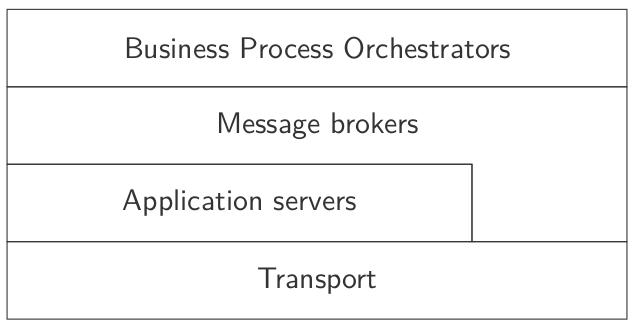
\includegraphics[scale=.3]{images/couches-middleware}
\caption{Niveaux d'abstraction du middleware}
\end{figure}

}

%--- 9 ----------------------------------------------------------
\item\qouv{Donnez la différence entre un client léger et lourd, dans une architecture client-serveur.}
{L'architecture client-serveur, de type distribuée, est constituée de deux sous-systèmes:
\begin{enumerate}
\item le \textbf{client}: émet des requêtes pour bénéficier des services du serveur
\item le \textbf{serveur}: reçoit les requêtes, les traite et envoie une réponse au client
\end{enumerate}

\paragraph{}
Ce modèle d'architecture peut être implémenté de différentes façons, selon l'importance que l'on donne au client:
\begin{itemize}
\item[$\cdot$] \textcolor{ltred}{\textsc{client léger}}: le client a peu de responsabilités, il interragit avec le serveur qui gère les données ET la logique applicative du système.
	\begin{figure}[h!]
	\center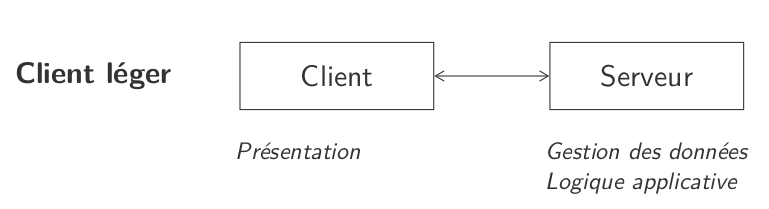
\includegraphics[scale=.3]{images/client-leger}
	\end{figure}
\item[$\cdot$] \textcolor{ltred}{\textsc{client lourd}}: la logique applicative est migrée du côté client, qui a désormais le plus grand rôle, laissant au serveur uniquement la gestion des données. Il faut imposer au client certaines capacités minimums pour faire fonctionner le système.
	\begin{figure}[h!]
	\center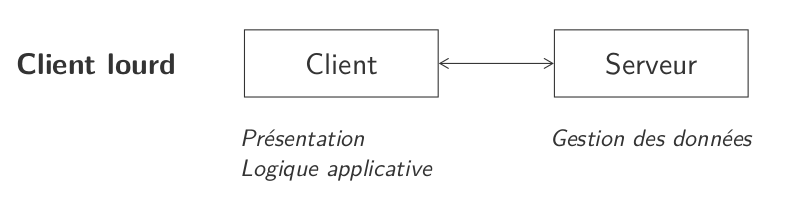
\includegraphics[scale=.3]{images/client-lourd}
	\end{figure}
\end{itemize}
}

%--- 10 ----------------------------------------------------------
\item\qouv{Qu’est-ce-que CORBA et quel type d’architecture supporte-t-il ?}
{}